%%%%%%%%%%%%%%%%%%%%%%%%%%%%%%%%%%%%%%%%%%%%%%%%
%
% figures - nothing too special here 
%
%%%%%%%%%%%%%%%%%%%%%%%%%%%%%%%%%%%%%%%%%%%%%%%%
\chapter{Figures}


% BASIC EXAMPLE
%================

\begin{figure}[h!tb]
\centering

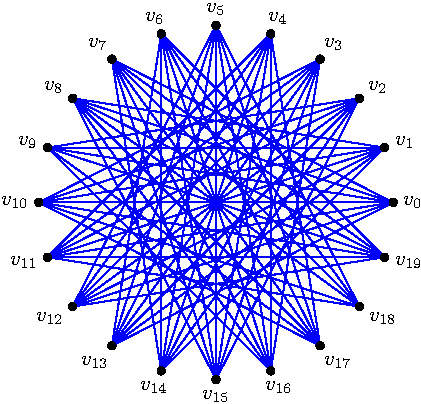
\includegraphics{example/figure} % not necessary to give extension - now you can shift between compiling to ps or to pdf without any problems
 
\caption[Do not end short caption with full-stop]{Each figure must be supplied with a long caption, making the figure stand-alone and ended with a full-stop.}

\end{figure}





\newpage





% SUBFIG EXAMPLE
%================
%
% usage: \subfloat[][caption]{...figure code...\label{label}}

The subfigures are Figures \subref{firstfigure}, \subref{secondfigure}, \subref{thirdfigure} and \subref{fourthfigure}.

\begin{figure}
\centering

\subfloat[][First subcaption (No full-stop)]{
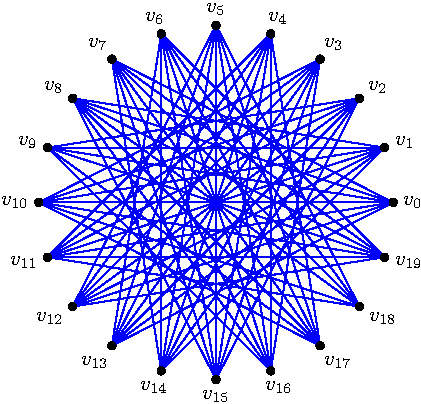
\includegraphics{example/figure}
\label{firstfigure}
}
\quad
\subfloat[][Second subcaption (No full-stop)]{
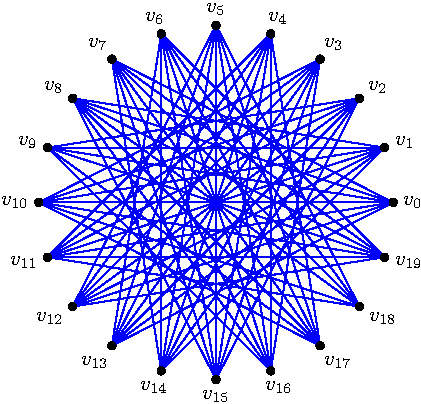
\includegraphics{example/figure}
\label{secondfigure}
}
\\
\subfloat[][Third subcaption (No full-stop)]{
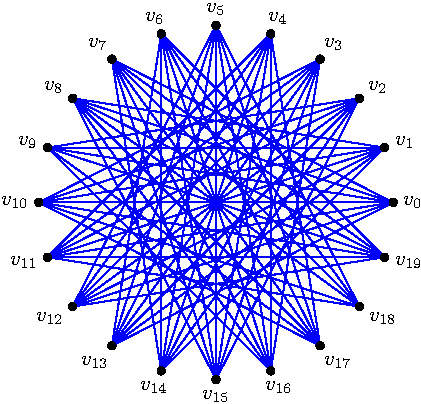
\includegraphics{example/figure}
\label{thirdfigure}
}
\quad
\subfloat[][Fourth subcaption (No full-stop)]{
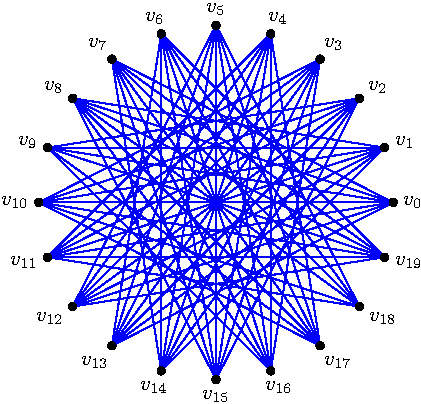
\includegraphics{example/figure}
\label{fourthfigure}
}
\caption[Do not end short caption with full-stop]{End the main caption with a full-stop, but not each of the sub-figure captions!}
\label{thislabel}
\end{figure}
